\subsection{Namespace Graph}\label{app:ns-detail}

The namespace graph $G_{\mathrm{ns}}^{(k)}$ (Definition~\ref{def:ns-graph}; \S\ref{sec:namespace-graph}) aggregates declarations by their position in the naming hierarchy, yielding a family of graphs parameterized by truncation depth~$k$. All statistics below use $k = 2$ unless noted otherwise.

\subsubsection{Containment Decay}

Table~\ref{tab:containment-decay} reports the containment ratio at each level of the namespace and module hierarchies.

\begin{table}[ht]
\centering
\caption[Containment across granularity levels]{Containment across granularity levels. Namespace-depth rows are computed on all $8{,}436{,}366$ edges of $G_{\mathrm{thm}}$. The top-level directory and file-level rows are computed on the $2{,}506{,}738$ edges whose both endpoints appear in the file-module mapping.\protect\footnotemark}
\label{tab:containment-decay}
\begin{tabular}{llrr}
\toprule
Granularity & Units & Cross-boundary & Containment \\
\midrule
Top-level directory             & $32$          & $51.1\%$ & $48.9\%$ \\
Namespace depth $1$             & $3{,}184$     & $77.8\%$ & $22.2\%$ \\
Namespace depth $2$             & $10{,}097$    & $85.8\%$ & $14.2\%$ \\
File-level                      & $7{,}225$     & $84.4\%$ & $15.6\%$ \\
Namespace depth $\ge 3$         & ${\sim}15$K   & $87.4\%$ & $12.6\%$ \\
\bottomrule
\end{tabular}
\end{table}
\footnotetext{The file-module mapping covers $217{,}647$ of $308{,}129$ declarations; unmapped declarations are primarily Lean core infrastructure residing outside the \texttt{Mathlib/} source tree.}

\begin{figure}[ht]
\centering

\includegraphics[width=\textwidth]{figures/containment_curve.pdf}
\caption{Containment decay curve. Green circles connected by the solid line show containment at namespace depth $k = 1, \ldots, 6$; blue squares mark file-system levels (top-level directory and file module). The gray dashed line marks the same-file baseline from Table~\ref{tab:thm-edge-breakdown} ($9.6\%$). Containment drops steeply from the top-level directory to depth~$1$ and saturates by depth~$3$.}
\label{fig:containment-curve}
\end{figure}

The decay exhibits three regimes. At the coarsest granularity---the $32$ top-level directories (\module{Algebra}, \module{CategoryTheory}, \module{Topology}, etc.)---nearly half of all declaration-level dependencies ($48.9\%$) stay within the same directory, confirming that discipline-level categories retain genuine organizational force. The steepest single drop occurs at the discipline--sub-discipline transition ($48.9\% \to 22.2\%$): moving from $32$ directories to $3{,}184$ depth-$1$ namespaces eliminates more than half of the remaining containment, indicating that within a discipline, boundaries between \ns{Nat} and \ns{Int}---or between \ns{Set} and \ns{Finset}---carry far less force. Beyond depth~$2$, containment barely decreases (from $14.2\%$ to $12.6\%$ at depth~$6$): finer naming distinctions add almost no intra-namespace edges. The file-module level ($7{,}225$ units, $15.6\%$ containment) falls between namespace depth~$1$ and depth~$2$, offering no containment advantage beyond that of a mid-level namespace.

\subsubsection{Degree Distribution}
\label{sec:ns-degree}

We examine the degree distribution of $G_{\mathrm{ns}}^{(2)}$, the namespace graph at depth~$2$. We choose $k = 2$ because it occupies the sweet spot of the containment decay curve (Table~\ref{tab:containment-decay}): depth~$1$ is too coarse ($3{,}184$ namespaces, comparable to the top-level directory partition), while depth~$3$ and beyond add almost no new cross-boundary structure (containment saturates at ${\sim}13\%$). At depth~$2$, the $10{,}097$ namespaces correspond to familiar mathematical groupings---\ns{Nat.Prime}, \ns{CategoryTheory.Functor}, \ns{MeasureTheory.Measure}---and provide enough nodes for meaningful network analysis. The graph has $332{,}081$ edges (unique namespace pairs), carrying a total weight of $7{,}234{,}844$ declaration-level dependencies.

\begin{table}[ht]
\centering
\caption{Degree statistics for $G_{\mathrm{ns}}^{(2)}$ (unweighted).}
\label{tab:ns-degree-stats}
\begin{tabular}{lrr}
\toprule
& In-degree & Out-degree \\
\midrule
Mean        & $32.9$    & $32.9$ \\
Median      & $1$       & $14$ \\
Std         & $223.2$   & $59.3$ \\
Max         & $9{,}846$ & $3{,}075$ \\
Zero-degree & $3{,}920$ & $6$ \\
\bottomrule
\end{tabular}
\end{table}

The degree distribution is extremely skewed (Table~\ref{tab:ns-degree-stats}). The median in-degree of~$1$ versus a mean of~$33$ reveals a long tail: $3{,}920$ namespaces ($38.8\%$) have zero in-degree---they are referenced by no other namespace---while a handful attract thousands of incoming edges. The top namespaces by in-degree are \ns{\_root\_} ($9{,}846$), \ns{Eq} ($7{,}686$), \ns{OfNat} ($4{,}390$), \ns{Membership} ($3{,}407$), and \ns{Semiring} ($3{,}252$). By out-degree, the leaders are \ns{\_root\_} ($3{,}075$), \ns{MeasureTheory} ($687$), \ns{CategoryTheory} ($656$), and \ns{Polynomial} ($615$).

Power-law fitting (\S\ref{sec:prelim-powerlaw}) yields $\alpha = 1.60$ ($x_{\min} = 4$) for in-degree and $\alpha = 1.90$ ($x_{\min} = 13$) for out-degree. In both cases, a lognormal distribution provides a significantly better fit than a pure power law (likelihood ratio $R = -10.6$ and $R = -289.7$, respectively; $p < 0.01$). This mirrors the pattern observed for $G_{\mathrm{module}}$ (\S\ref{sec:degree-distribution}): heavy-tailed distributions that are not cleanly power-law.

\begin{figure}[ht]
\centering

\includegraphics[width=\textwidth]{figures/ns_degree_distribution.pdf}
\caption{Degree distributions of $G_{\mathrm{ns}}^{(2)}$ on log--log axes. Left: in-degree (\textcolor{blue!60!black}{blue}), with power-law reference (gold dashed, $\alpha = 1.60$, $x_{\min} = 4$). Right: out-degree (\textcolor{red!60!black}{coral}), with power-law reference ($\alpha = 1.90$, $x_{\min} = 13$). Both tails are heavy but better fit by a lognormal than a pure power law. The extreme outlier in the in-degree panel is \ns{\_root\_} ($\deg^{-} = 9{,}846$; see Remark~\ref{rem:root-artifact}).}
\label{fig:ns-degree}
\end{figure}

\label{rem:root-artifact}
The namespace \ns{\_root\_} dominates both in-degree and out-degree at depth~$2$. This is an artifact of the truncation rule in Definition~\ref{def:ns-graph}: declarations whose fully qualified names have fewer than three components---including foundational definitions such as \decl{Eq.refl}, \decl{Nat.succ}, and \decl{OfNat.ofNat}---are assigned to \ns{\_root\_}. This namespace is not a coherent conceptual domain; it is a catch-all for the shallow infrastructure of the Lean type system. Its extreme centrality reflects naming-depth convention rather than mathematical importance: the most foundational constructs carry the shortest names. In the analysis that follows, we note where \ns{\_root\_} distorts aggregate statistics.

As at the module (\S\ref{sec:degree-distribution}) and declaration (\S\ref{sec:thm-degree}) levels, the degree distributions are heavy-tailed but better fit by lognormal than pure power law. In-degree skewness is extreme (median~$1$ vs.\ mean~$33$), distorted by the \ns{\_root\_} artifact (Remark~\ref{rem:root-artifact}). The in-degree/out-degree asymmetry mirrors the pattern at the other two levels: open-ended in-degree (product) versus bounded out-degree (process).

\subsubsection{DAG Depth}
\label{sec:ns-dag-depth}

Unlike $G_{\mathrm{module}}$ and $G_{\mathrm{thm}}$, the namespace graph $G_{\mathrm{ns}}^{(2)}$ is \emph{not} a DAG: aggregating declaration-level dependencies to the namespace level creates cycles (e.g., \ns{Nat} $\to$ \ns{Int} $\to$ \ns{Nat}), because declarations in different namespaces can depend on each other bidirectionally (Remark~\ref{rem:ns-cycles}). To recover a layered structure, we condense strongly connected components (SCCs), yielding a DAG of $4{,}080$ super-nodes in $8$ topological layers. The structure is bimodal: layer~$0$ contains $3{,}941$ super-nodes (mostly trivial, single-namespace SCCs that depend on nothing else), while layer~$5$ contains a single super-node---the giant SCC of $5{,}899$ namespaces ($58\%$ of all depth-$2$ namespaces). The intermediate layers ($1$--$4$) hold only $134$ super-nodes that bridge the leaf namespaces to the giant core. Beyond the giant SCC, layers~$6$ and~$7$ contain just $4$ namespaces.

\begin{figure}[ht]
\centering

\includegraphics[width=\textwidth]{figures/ns_dag_structure.pdf}
\caption{Condensed DAG of $G_{\mathrm{ns}}^{(2)}$ by topological layer ($4{,}080$ super-nodes, $8$ layers). Each bar counts the number of super-nodes (SCCs) at that layer. Layer~$0$ holds $3{,}941$ leaf SCCs; layer~$5$ holds a single giant SCC comprising $5{,}899$ namespaces. The shallow, bimodal structure reflects pervasive mutual dependency: most namespaces either sit at the periphery or belong to one densely interconnected core.}
\label{fig:ns-dag-structure}
\end{figure}

The $8$-layer condensed DAG is far shallower than the module ($154$) or declaration ($84$) graphs: at the namespace level, pervasive mutual dependency produces a nearly flat structure rather than vertical hierarchy.

\subsubsection{Centrality}
\label{sec:ns-centrality}

As in \S\ref{sec:centrality} and \S\ref{sec:thm-centrality}, we compute PageRank and betweenness centrality (Definition~\ref{def:pagerank}--\ref{def:betweenness}; $\alpha = 0.85$, weighted; $k = 300$ samples) to identify structurally important namespaces.

\begin{table}[ht]
\centering
\caption{Top~10 namespaces by PageRank and betweenness centrality in $G_{\mathrm{ns}}^{(2)}$.}
\label{tab:ns-centrality}
\small
\begin{tabular}{rlrl}
\toprule
\multicolumn{2}{c}{PageRank} & \multicolumn{2}{c}{Betweenness} \\
\cmidrule(lr){1-2} \cmidrule(lr){3-4}
PR & Namespace & $c_B$ & Namespace \\
\midrule
.247 & \ns{\_root\_}          & .248 & \ns{\_root\_} \\
.035 & \ns{Eq}                & .065 & \ns{And} \\
.017 & \ns{Set}               & .043 & \ns{Eq} \\
.015 & \ns{Iff}               & .036 & \ns{Exists} \\
.014 & \ns{OfNat}             & .031 & \ns{Function} \\
.012 & \ns{Real}              & .030 & \ns{Nat} \\
.012 & \ns{Nat}               & .029 & \ns{CategoryTheory} \\
.012 & \ns{CategoryTheory}    & .019 & \ns{MeasureTheory} \\
.010 & \ns{Preorder}          & .018 & \ns{Set} \\
.008 & \ns{Semiring}          & .017 & \ns{Module} \\
\bottomrule
\end{tabular}
\end{table}

Excluding the \ns{\_root\_} artifact (Remark~\ref{rem:root-artifact}), the two rankings reveal a clear separation (Table~\ref{tab:ns-centrality}). PageRank is dominated by mathematical infrastructure: \ns{Eq}, \ns{Set}, \ns{OfNat}, \ns{Real}, and \ns{Preorder}---the foundational types and structures on which proofs ultimately rest. Betweenness centrality, by contrast, promotes logical connectives and bridging concepts: \ns{And}, \ns{Exists}, and \ns{Function} occupy positions~$2$--$5$ by betweenness but do not appear in the PageRank top~$10$. These namespaces serve as structural bridges: proofs in distant mathematical theories must pass through logical connectives to compose their arguments.

This separation echoes the module-level finding of \S\ref{sec:centrality}, where no single module dominates all three centrality measures, and the declaration-level finding of \S\ref{sec:thm-centrality}, where in-degree, PageRank, and betweenness identify disjoint categories of importance. At the namespace level, the two available measures already diverge sharply, confirming that the multidimensionality of structural importance persists across all three granularities. Figure~\ref{fig:ns-centrality} shows the pairwise scatter plots.

\begin{figure}[H]
\centering
\begin{subfigure}[t]{0.32\textwidth}
\centering
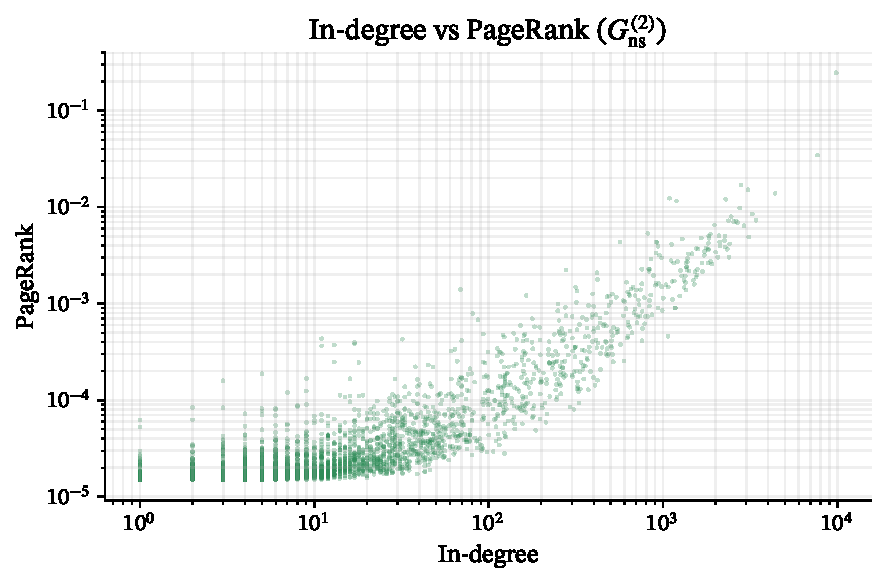
\includegraphics[width=\textwidth]{figures/ns_centrality_indeg_pr.pdf}
\caption{In-degree vs.\ PageRank.}
\label{fig:ns-centrality-indeg-pr}
\end{subfigure}%
\hfill
\begin{subfigure}[t]{0.32\textwidth}
\centering
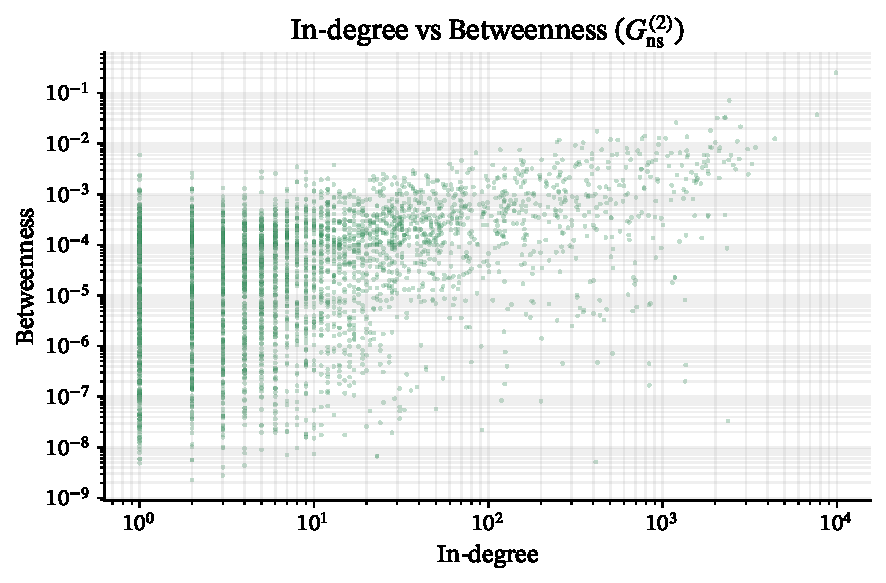
\includegraphics[width=\textwidth]{figures/ns_centrality_indeg_betw.pdf}
\caption{In-degree vs.\ Betweenness.}
\label{fig:ns-centrality-indeg-betw}
\end{subfigure}%
\hfill
\begin{subfigure}[t]{0.32\textwidth}
\centering

\includegraphics[width=\textwidth]{figures/ns_centrality_betw_pr.pdf}
\caption{Betweenness vs.\ PageRank.}
\label{fig:ns-centrality-betw-pr}
\end{subfigure}
\caption{Pairwise centrality scatter plots for $G_{\mathrm{ns}}^{(2)}$. Each point is one namespace. The extreme outlier in (a) is \ns{\_root\_} (Remark~\ref{rem:root-artifact}). The scatter confirms that PageRank and betweenness capture distinct structural roles at the namespace level.}
\label{fig:ns-centrality}
\end{figure}

\subsubsection{Community Structure}
\label{sec:ns-community}

Louvain community detection (\S\ref{sec:prelim-community}) on the undirected, weighted projection of $G_{\mathrm{ns}}^{(2)}$ yields $12$ communities with modularity $Q = 0.270$.

\begin{table}[ht]
\centering
\caption{Top five communities in $G_{\mathrm{ns}}^{(2)}$ by size, with representative namespaces (highest weighted in-degree within each community).}
\label{tab:ns-communities}
\begin{tabular}{rrl}
\toprule
ID & Size & Representative namespaces \\
\midrule
3 & $5{,}096$ & \ns{\_root\_}, \ns{Set}, \ns{Nat} \\
5 & $2{,}227$ & \ns{Semiring}, \ns{NonUnitalNonAssocSemiring}, \ns{DFunLike} \\
4 & $1{,}363$ & \ns{Eq}, \ns{CategoryTheory}, \ns{CategoryTheory.Functor} \\
0 & $1{,}041$ & \ns{Real}, \ns{Zero}, \ns{Field} \\
1 & $360$     & \ns{DivInvMonoid}, \ns{MulOne}, \ns{MulOneClass} \\
\bottomrule
\end{tabular}
\end{table}

The namespace-level community structure differs markedly from the declaration-level structure (\S\ref{sec:thm-community}). At the declaration level, Louvain detection produces $22$ communities with modularity $0.48$ and NMI~$= 0.34$ against the top-level namespace hierarchy. At the namespace level, the number of communities is smaller ($12$ vs.\ $22$), the modularity is lower ($0.270$ vs.\ $0.48$), and the NMI with the top-level directory falls to~$0.243$ (Table~\ref{tab:ns-communities}).

The lower modularity reflects the coarsening inherent in namespace aggregation. When thousands of declarations are collapsed into a single namespace node, the fine-grained community boundaries that Louvain detects at the declaration level are blurred. Edges between namespaces are weighted sums of many declaration-level edges, and the averaging effect smooths out the modular structure that exists at finer granularity. The largest community (ID~$3$, $5{,}096$ nodes) spans half the graph and lacks a coherent mathematical identity: its dominant members (\ns{\_root\_}, \ns{Set}, \ns{Nat}) are foundational constructs used across all disciplines. This contrasts with the declaration-level communities, where the largest communities map onto recognizable mathematical disciplines (\S\ref{sec:thm-community}).



\subsubsection{Robustness}
\label{sec:ns-robustness}

We assess the robustness of $G_{\mathrm{ns}}^{(2)}$ by progressively removing nodes and measuring the fraction of the original graph remaining in the largest weakly connected component (GCC). The original graph has $4$ weakly connected components, with the largest containing $10{,}094$ of $10{,}097$ nodes.

\begin{table}[ht]
\centering
\caption{Robustness of $G_{\mathrm{ns}}^{(2)}$: GCC fraction after random vs.\ targeted (PageRank-ordered) node removal.}
\label{tab:ns-robustness}
\begin{tabular}{rrrr}
\toprule
Removal \% & Random GCC & Targeted GCC & Gap \\
\midrule
$5\%$  & $0.950$ & $0.726$ & $0.223$ \\
$10\%$ & $0.899$ & $0.509$ & $0.391$ \\
$20\%$ & $0.798$ & $0.208$ & $0.590$ \\
$30\%$ & $0.688$ & $0.054$ & $0.634$ \\
$50\%$ & $0.477$ & $0.000$ & $0.477$ \\
\bottomrule
\end{tabular}
\end{table}

\begin{figure}[ht]
\centering
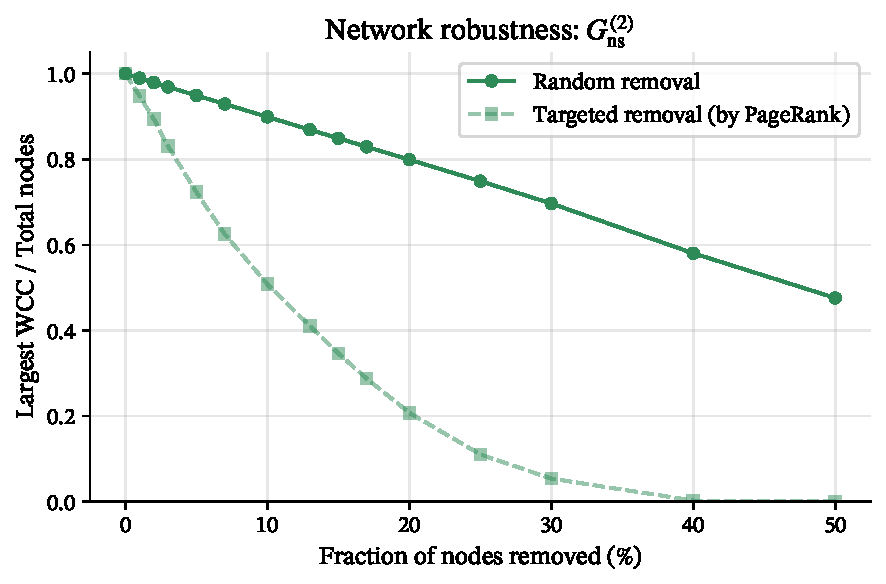
\includegraphics[width=\textwidth]{figures/ns_robustness_curve.pdf}
\caption{Robustness curves for $G_{\mathrm{ns}}^{(2)}$: fraction of nodes in the largest WCC as a function of the fraction removed, under random removal (blue) and targeted removal by PageRank (coral).}
\label{fig:ns-robustness}
\end{figure}

The pattern matches the classic hub-dominated vulnerability signature observed at both the module level (\S\ref{sec:robustness}) and the declaration level (\S\ref{sec:thm-robustness}): high resilience under random failure, extreme fragility under targeted attack (Table~\ref{tab:ns-robustness}, Figure~\ref{fig:ns-robustness}). At $20\%$ targeted removal, the GCC collapses to $20.8\%$ of its original size---more severe than the declaration-level graph, where the same removal fraction leaves $46.1\%$ (\S\ref{sec:thm-robustness}). The namespace graph's greater fragility reflects the concentration of connectivity in the \ns{\_root\_} super-node and a small number of infrastructure namespaces (Remark~\ref{rem:root-artifact}); once these are removed, the remaining mathematical namespaces fragment into isolated clusters with no shared foundation.

\subsubsection{Extended Analysis}\label{app:ns-analysis}

The containment decay curve (Figure~\ref{fig:containment-curve}) measures how well the namespace hierarchy captures dependency structure. The disciplinary taxonomy---Algebra, Analysis, Topology, Number Theory---retains genuine organizational force at the broadest scale, but this force dissipates rapidly at the sub-discipline transition ($48.9\% \to 22.2\%$). Within a discipline, boundaries between \ns{Nat} and \ns{Int} carry far less constraining power than the boundary between \ns{Algebra} and \ns{Topology}. The saturation beyond depth~$2$ (${\sim}13\%$) suggests the namespace tree is ``informationally shallow'': its first two levels encode most dependency structure that human naming captures, and deeper levels serve primarily as disambiguation.

The heightened fragility of the namespace graph under targeted attack (GCC reduced to $20.8\%$ at $20\%$ removal, versus $46.1\%$ at the declaration level) arises because namespace aggregation concentrates dependencies: a handful of infrastructure namespaces---\ns{Eq}, \ns{OfNat}, \ns{DFunLike}---absorb thousands of declaration-level dependencies into single namespace-level hubs. Refactoring such bottleneck namespaces carries disproportionate systemic risk and should be guided by centrality rankings.

